\documentclass{article}
\usepackage{geometry}
\usepackage{amsmath,amssymb}
\usepackage{graphicx}
\title{Mean Job access delay under Coding and Replication schemes in Storage systems}
\author{Raghuram Bharadwaj, Gokul Nair}

\begin{document}
	\maketitle
	\section{Introduction}
	Large server data centres are very important in today's world and their ubiquity needs no introduction. To reliably store these files there are several techniques that can be adopted, of which two important ones are replication and coding. The former is the introduction of redundancy in the system, where a file is saved in multiple copies at different servers, while the latter involves a clever way of dividing the file into chunks and storing it such that access to some (not all) chunks allows the requester to construct the entire file. For example, if we say that coding scheme is (n,k), we mean that a file is divided into $n$ codes and stored in $n$ servers. Any $k$ chunks are enough to decode and reconstruct the entire file. Now the natural question to ask is which of the two techniques minimizes the mean job access delay. In \cite{imppaper}, authors provided analysis showing that the coding scheme is better both when the arrival rate is very small and very large. The assumption made in the paper is that the arrival rates of all the files are same. In this case, they showed that as $k$ increases, the mean job access delay decreases. In the current work, we want to analyse the mean job access delay when the arrival rates of files are different. In this case, we want to find the right coding scheme, i.e., value of $n_{i}$ and $k_{i}$ for each file $i$, so that the mean job access delay is minimized. 
	
\section{Organisation of the Report}
We first discuss the problem model and the analysis in the paper \cite{imppaper} and perform simulations. To get better understanding, we extend the simulations to the case where service rates of files are different. In Section 5, we analyse the mean job access delay, when arrival rates of all files are not same but have the same coding scheme $(n,k)$. Finally in Section 6, we attempt to analyse the mean job access delay when each file has different coding scheme. In Section 7, we provide concluding remarks followed by future work. 

\section{The Model}

In the coding scheme, when the file is divided into $ n $ chunks, such that knowledge of $ k $ chunks allows for its reconstruction, the notation used is $ (n,k) $. In this notation the n-replication scheme is $ (n,1) $.\\

The system consists of $ L $ servers and they store a multitude of files according to the MDS code. The number of files stored on the system is $ I $, and the arrival process is modelled as a Poisson process with rate $ \lambda $, $ \lambda\in (0,1) $, at each server $L$. Therefore, the overall arrival rate is $L\lambda$. The time to download the complete file is i.i.d exponential with rate $1$. Therefore in the coding scheme, the time to download a chunk from each server is exponential with rate $k$.  Each arrival entails a request for  one of the $ I $ files uniformly. To minimise the delay in the system a `load balance' algorithm is to be adopted. Each server has an infinite buffer where it queues requests for chunks and responds to them in the FIFO manner. When a file request arrives to a $ (n,k) $ system, there are $ n $ possible servers who can help of which $ k $ are enough to retrieve the file. The algorithm adopted is to send the request to the $k$ least occupied queues. 
\medskip

\begin{equation}
\bar{W}^{(n,k)}:= \text{Mean time to access time for file in the (n,k) scheme}.
\label{1}
\end{equation}

\begin{equation}
\bar{W}^{(nk,k)}=\mathbb{E}\left[ \text{max}_{i=1,2,..k} X_i \right]
\label{2}
\end{equation}
Where $\{ X_i \}$ are i.i.d. exponentially distributed random variables with parameter $ k $. Equation \eqref{2} follows since to retrieve a file we need $ k $ chunks and the time to retrieve these chunks is determined by the one that takes maximum time.

\subsection{Analysis}
The main step in analysing the mean job access delay is to obtain the distribution of number of jobs waiting at each server. In general, the number of jobs at each server is dependent on that at other servers. But if we make the mean field assumption, i.e., $ L\rightarrow \infty $, then the distribution of number of jobs at each server becomes i.i.d. So, in this scenario, it is enough to focus our analysis on single server. Therefore, let 

\begin{equation}
Q^{L}_l(t):= \text{Length of } l^{th} \text{queue in a system of L servers.}
\label{3}
\end{equation} 

It can be shown that the vectors $\{ Q^{L}(t)\} $ is a positive recurrent Markov Chain with steady state distribution. Due to the symmetry in the problem, all the queues have the same steady state distribution. $ \bar{\pi}_m := P\{\bar{Q}^{(n,k)} = m\}  $, where $ \bar{Q}^{(n,k)} $ is a random variable equal in distribution to the steady state queue length. Let $q_{m,m+1}$ be the transition rate to go from $m$ to $m+1$.  The reverse rate is $ k $, as it is the service rate of each code and length of queue decreases by 1 after the service. Hence, we can write detailed balanced equations as: 
\begin{equation}
\bar{\pi}_mq_{m,m+1}=k\bar{\pi}_{m+1}
\end{equation}

If we know the value of $q_{m,m+1}$, then we can compute the distribution of number of waiting jobs at the server. But it's difficult to directly compute this value. So, we approach this derivation in other way. The average number of servers that have length $m$ is $L\pi_{m}$. Therefore, number of servers that move from $m$ to $m+1$ length in a small time interval $ \tau $, is given by $L\pi_{m}q_{m.m+1}\tau$. Another way of approaching to this expression is the following. $ L\lambda\tau$ customers arrive in time $\tau$ of which $ L\lambda\sum_{i=1}^{k}P\{\bar{Q}^{(n,k)}_{(i)}=m\}\tau$ join queues with size $ m $. Here $\bar{Q}^{(n,k)}_{(i)}$ is the $ i^{th} $ smallest queue among those $ n $ servers which contain chunks of the file being requested. This expression can be derived easily by considering the load balance algorithm: a request joins a queue of length $ m $ only if it is one of the $ k $ smallest available queues. These queues increase their size from $ m $ to $ m+1 $. Equating the two expressions:
\begin{equation}
\bar{\pi}_mq_{m,m+1}=\lambda \sum_{i=1}^{k}P\{\bar{Q}^{(n,k)}_{(i)}=m\}
\end{equation}
Using this, we obtain a recurrence relation for the steady state queue length of a single server:
\begin{equation}\label{dist}
\bar{s}_{m+1}=\lambda \frac{f^{(n,k)}(\bar{s}_{m})}{k} \text{ for } m=0,1,2...\\
\end{equation}

\begin{equation}
\bar{s}_{0}=1
\end{equation}
Where $ f^{(n,k)}(x) = \sum_{l=1}^{k} {{n}\choose{n-k+l}}{{n-k+l-2}\choose{l-1}}(-1)^{l-1}x^{n-k+l} $ for $ x\in [0,1] $.
\medskip

The next step is to find the mean job access delay. To completely retrieve a file, $ k $ servers have to let their requests through. Each queue will already have $ \bar{Q}^{(n,k)}_{(i)} $ requests in line. Each of these requests will take $ X^{(k,i)}\sim\text{exp}(k)$ time to process plus its own processing time. The mean delay experienced by the request will be:
\begin{equation} \label{delay}
\bar{W}^{(n,k)} = \mathbb{E}\left[ \text{max}_{i=1,2,..k} \sum_{j=1}^{\bar{Q}^{(n,k)}_{(i)}+1}X_j^{(k,i)} \right]
\end{equation}

In this way, we can compute the mean job access delay.

\section*{\huge Our Work}

\section{Simulation Results}
In this section, we simulated the above analysis. For the coding scheme $(n,k)$, we first generated $n$ i.i.d queue-length random variables according to \eqref{dist}. Then we selected $k$ least length queue-lengths and calculated job delay according to \eqref{delay}. The MATLAB code for this simulation is included in the folder.

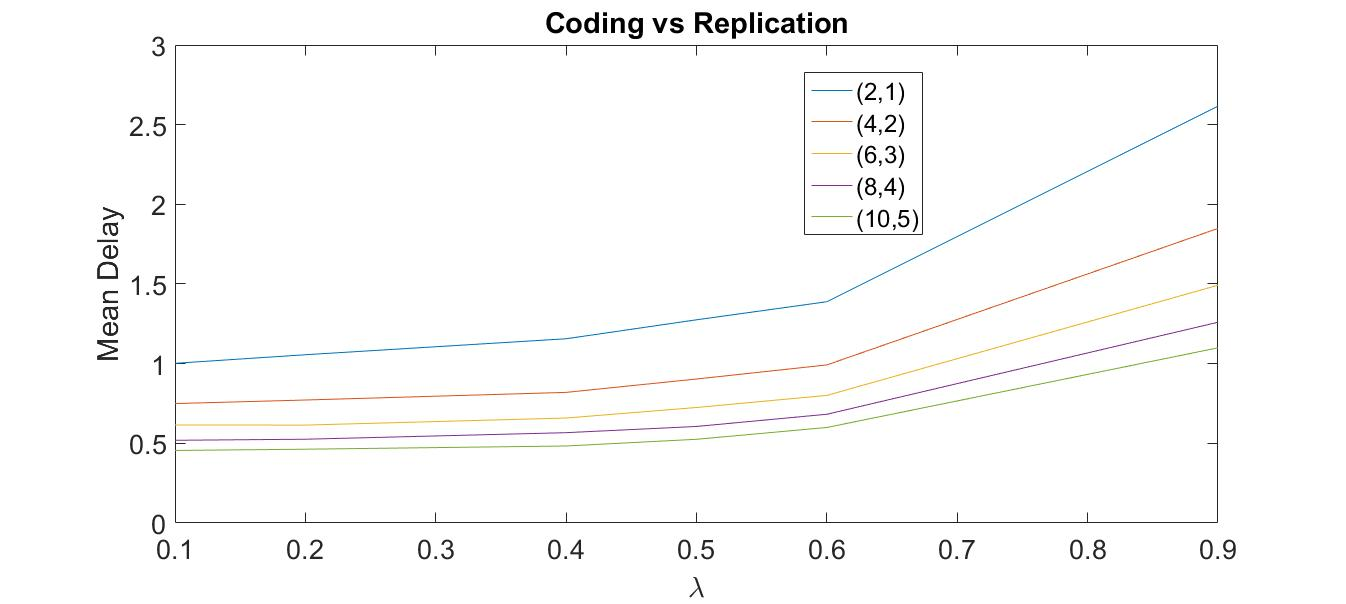
\includegraphics[width = 15cm, height = 8cm]{result1.jpg}

\subsection{Different Service Rates}

In this section, we classified jobs into 2 categories. The service time for jobs of category 1 is exponential with mean $1.5$. The service time for jobs of category 2 is exponential with mean $0.5$.
Both the categories of jobs occur with same probability. These values are selected as these do not disturb the previous analysis and the derived formulae can be directly applied. This is because, rate at which a server will now move from $m+1$ to $m$ under $(n.k)$ coding scheme will be: 
$$ 1/2*(1.5/k + 0.5/k) =  1/k, $$ which is same as in previous case. 

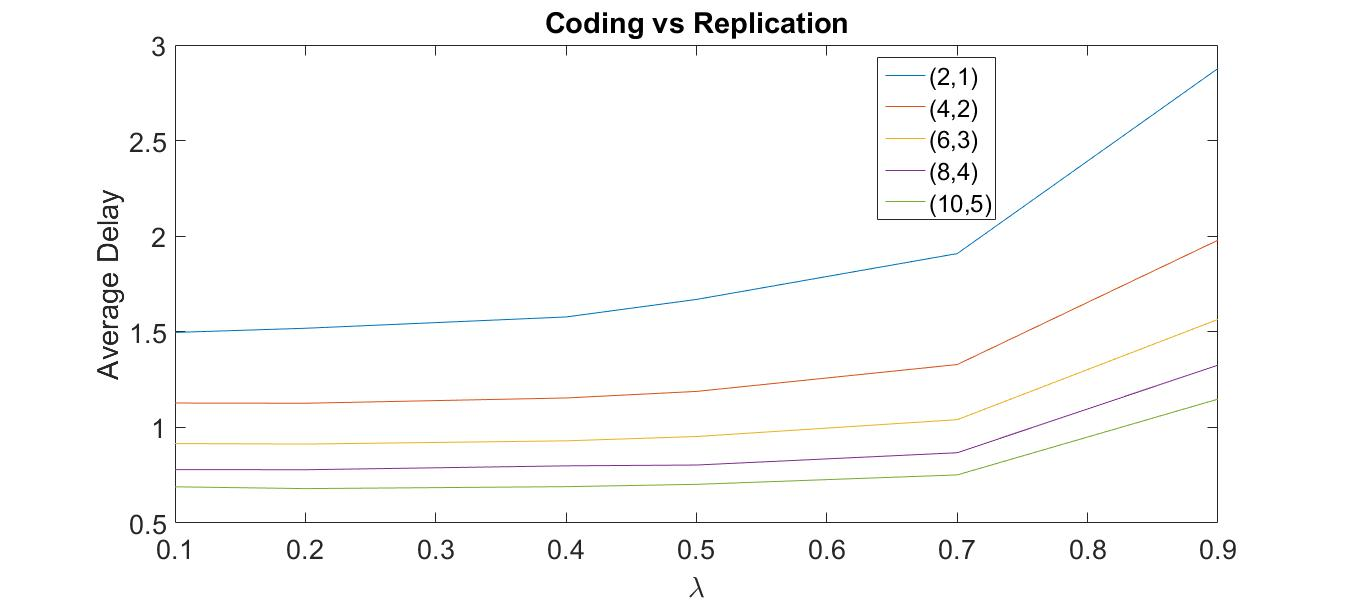
\includegraphics[width = 15cm, height = 8cm]{result2.jpg}

\subsection{Observations}
\begin{itemize}
	\item We observe that mean file access delay improves as the value of $k$ increases, which reiterates the idea that coding scheme is better than replication.
	\item As the arrival rate increase, we observe that delay increases. This is because, as the rate increases, the mean time between arrivals decreases, and hence there will be more jobs at each server, increasing the job delay.
	\item So we observe that in the case where arrival rates of all the files are the same, as value of $k$ increases, the delay decreases. 
\end{itemize}

In the next section, we wish to analyse the mean job delay when the arrival rates of files are all not same. We first analyse the case where all the files follow the same coding scheme and in the subsequent section, we extend it to the case where files have different coding schemes. 

\section{Files with different arrival rates under same coding scheme $(n,k)$}

Let the arrival rate of file $i$ be $\lambda_{i}$. Let $I_{j}$ be a set denoting the files, whose codes have been stored at server $j$. As before, the first step is to obtain the steady state queue-length distribution.

We can analyse the above system by letting the state at any time to be the queue-length at each server. That is state will be $n = (n_{1},n_{2},n_{3},.....)$. The process of successive states will be a Continuous-Time Markov Chain. 

Let $n_{i}^{*} = (n_{1},n_{2},....,n_{i}+1,n_{i+1},...)$. To go from $n$ to $n_{i}^{*}$, a new request must occur at the server $i$, and the server is one of $k$ least occupied servers. To analyse this system, we assume that the probability that a server is one of least $k$ occupied is $k/n$. Now we can use the time-reversibility equations to write the following:

\begin{equation} \label{reverse}
\pi(n)*(k/n)*\sum_{i \in I_{i}}\lambda_{i} = \pi(n_{i}^{*})*k 
\end{equation} 

Let the limiting probabilities, under mean-filed assumption satisfy 

$$ \pi(n_{1},n_{2},...) = \pi_{1}(n_{1})*\pi_{2}(n_{2})*....$$

Then \eqref{reverse} reduces to :

$$ \pi_{i}(n_{i})*(k/n)*\sum_{i \in I_{i}}\lambda_{i}  = \pi_{i}(n_{i}+1)*(k) $$. 

We solve this equation and the solution is as follows:

\begin{equation}\label{soln}
\pi_{i}(n) = (\sum_{i \in I_{i}}\lambda_{i}/n)^{n} * (1 - \sum_{i \in I_{i}}\lambda_{i}/n).
\end{equation}

Thus using \eqref{soln}, we can compute the steady-state queue length distribution. Then we can use \eqref{delay} to compute the mean job access delay. 

\section{Files with different arrival rates and different coding schemes}

The difference in this system is that each file is coded differently. The advantage of this model is that it helps us in identifying the right configuration. In the current work, however, we assume that files are assigned a coding model. Let file $i$ be coded with $(n_{i},k_{i})$ scheme. The analysis is similar to the one above and hence we can write time reversible equations as follows:

$$
\pi_{i}(n_{i})*\sum_{i \in I_{i}}(k_{i}/n_{i})*\lambda_{i}  = \pi_{i}(n_{i}+1)*\sum_{i \in I_{i}} (\lambda_{i}/\sum_{i \in I_{i}}\lambda_{i}) *k_{i}
$$

The above equation is obtained as follows. The queue length at server $i$ increases by 1, when a request arrives at $i$ and it is one of least occupied servers. As each file has its own coding, probability that server is one of the $k_{i}$ least occupied server for request $i$ is $k_{i}/n_{i}$. Now, for reversible process, we first need to know, the job that is at the beginning of the queue. In current work, we consider the probability that the job $i$ is at the beginning of the server is directly proportional to its arrival rate and hence the above equation. 

We solve the above equation and we obtain: Let $\sum_{i \in I_{i}} \lambda_{i} = \Lambda$

$$
\pi_{i}(n) = (\sum_{i \in I_{i}} (\lambda_{i}*k_{i}/\Lambda )/(\sum_{i \in I_{i}} k_{i}*\lambda_{i}/n_{i}))^{n}*(1 - \sum_{i \in I_{i}} (\lambda_{i}*k_{i}/\Lambda )/(\sum_{i \in I_{i}} k_{i}*\lambda_{i}/n_{i}))
$$

Thus, we compute the steady-state distribution in this model and then compute the mean job access delay as in \eqref{delay}.

\section{Conclusion}

In the current work, we first described the model of queueing system, where files are stored and accessed by replication and coding schemes. We then discussed the analysis in \cite{imppaper} that showed that the coding scheme outperforms replication, in case where all the files have same arrival rates. We performed simulations and verified the results. Then we performed similar analysis in cases where files have different arrival rates and then files that were coded under different coding schemes. 

\section{Future Work}
In Section 5 and 6, the analysis we did is based on approximations and would like to improve the analysis. Furthermore, we can extend our work to find the optimal coding scheme $(n_{i},k_{i})$ for each file $i$.

\begin{thebibliography}{9}
	\bibitem{imppaper} 
	Li, Bin and Ramamoorthy, Aditya and Srikant, R
	\textit{Mean-field-analysis of coding versus replication in cloud storage systems}. 
	Computer Communications, IEEE INFOCOM 2016-The 35th Annual IEEE International Conference, 2016
\end{thebibliography}









 



 



	  
	
	
\end{document}